% Auto-generated on 2026-03-01 from four skill folders only.
% Suggested packages in preamble:
% \usepackage{booktabs,threeparttable,siunitx,xcolor,pgfplots}
% \pgfplotsset{compat=1.18}

\subsection{Skill Distribution Overview}
\paragraph{Computation protocol.}
All statistics are computed by scanning \texttt{SKILL.md} files under exactly four folders: \texttt{chinese\_gpt3.5\_8}, \texttt{english\_gpt3.5\_8}, \texttt{chinese\_gpt4\_8}, and \texttt{english\_gpt4\_8}. The corpus/category counts in Tables~\ref{tab:autoskill-corpus-scale}--\ref{tab:autoskill-category-dist} and Figures~\ref{fig:autoskill-category-bars}--\ref{fig:autoskill-platform-bars} are absolute frequencies over these files, and percentages are normalized by the total number of skills ($N=1858$), i.e., $\mathrm{Share}(\%) = \frac{\mathrm{count}}{1858}\times 100$. Top tags are obtained from YAML \texttt{tags} fields with case-insensitive normalization for Latin tags (e.g., \texttt{Python}/\texttt{python} merged), while platform mentions are counted if platform keywords appear in skill name/description/tags/triggers.

\begin{table}[t]
\centering
\small
\begin{threeparttable}
\begin{tabular}{lrrr}
\toprule
Corpus & Skills & Share (\%) & Cumulative (\%) \\
\midrule
chinese\_gpt3.5\_8 & 400 & 21.53 & 21.53 \\
english\_gpt3.5\_8 & 631 & 33.96 & 55.49 \\
chinese\_gpt4\_8 & 224 & 12.06 & 67.55 \\
english\_gpt4\_8 & 603 & 32.45 & 100.00 \\
\midrule
\textbf{Total} & \textbf{1858} & \textbf{100.00} & \textbf{--} \\
\bottomrule
\end{tabular}
\caption{Skill counts across the four analyzed folders.}
\label{tab:autoskill-corpus-scale}
\end{threeparttable}
\end{table}

\begin{table}[t]
\centering
\small
\begin{threeparttable}
\begin{tabular}{lrr}
\toprule
Category & Skills & Share (\%) \\
\midrule
Programming \& Software Dev. & 482 & 25.94 \\
Writing \& Content Creation & 363 & 19.54 \\
Data \& AI/ML & 354 & 19.05 \\
Systems / DevOps / Config & 194 & 10.44 \\
Research \& Education & 72 & 3.88 \\
Operations \& Marketing & 23 & 1.24 \\
Other Domain-Specific & 14 & 0.75 \\
General / Mixed & 356 & 19.16 \\
\midrule
\textbf{Total} & \textbf{1858} & \textbf{100.00} \\
\bottomrule
\end{tabular}
\caption{Category distribution of extracted skills.}
\label{tab:autoskill-category-dist}
\end{threeparttable}
\end{table}

\begin{table}[t]
\centering
\small
\begin{threeparttable}
\begin{tabular}{rlr}
\toprule
Rank & Normalized Tag & Frequency \\
\midrule
1 & python & 98 \\
2 & javascript & 38 \\
3 & excel & 36 \\
4 & c++ & 35 \\
5 & creative writing & 35 \\
6 & formatting & 35 \\
7 & pandas & 30 \\
8 & education & 29 \\
9 & translation & 28 \\
10 & matlab & 24 \\
11 & automation & 24 \\
12 & pytorch & 23 \\
13 & java & 21 \\
14 & json & 21 \\
15 & roleplay & 20 \\
\bottomrule
\end{tabular}
\caption{Top normalized tags (case-insensitive for Latin tags).}
\label{tab:autoskill-top-tags}
\end{threeparttable}
\end{table}

\begin{figure}[t]
\centering
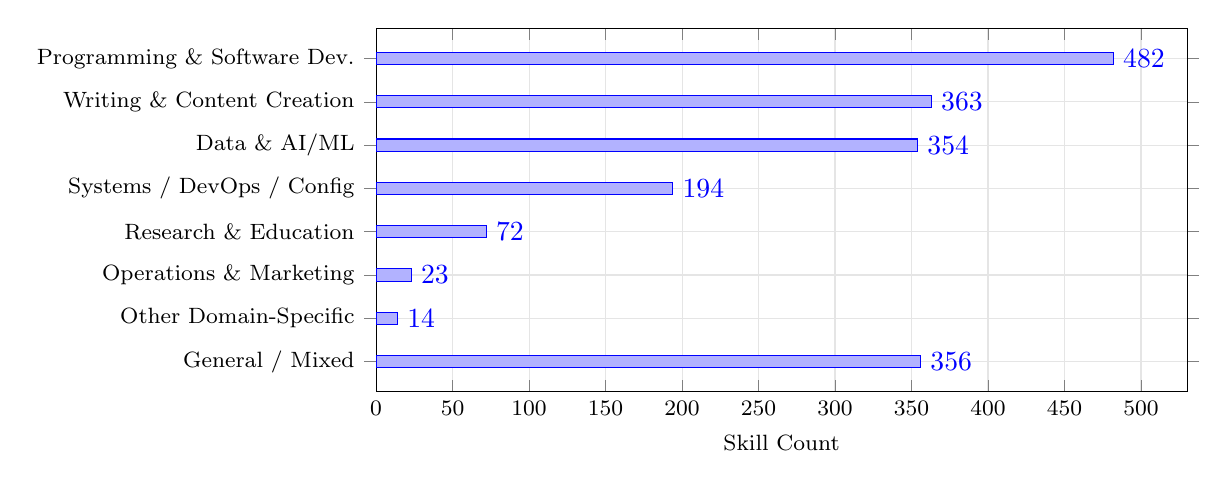
\begin{tikzpicture}
\begin{axis}[
width=0.98\linewidth,
height=6.2cm,
xbar,
xmin=0,
xlabel={Skill Count},
symbolic y coords={Programming \& Software Dev.,Writing \& Content Creation,Data \& AI/ML,Systems / DevOps / Config,Research \& Education,Operations \& Marketing,Other Domain-Specific,General / Mixed},
ytick=data,
y dir=reverse,
bar width=4.4pt,
nodes near coords,
nodes near coords align={horizontal},
tick label style={font=\footnotesize},
label style={font=\footnotesize},
grid=major, grid style={draw=gray!20},
every axis plot/.append style={fill=blue!55, draw=blue!80!black},
]
\addplot coordinates {
(482,Programming \& Software Dev.)
(363,Writing \& Content Creation)
(354,Data \& AI/ML)
(194,Systems / DevOps / Config)
(72,Research \& Education)
(23,Operations \& Marketing)
(14,Other Domain-Specific)
(356,General / Mixed)
};
\end{axis}
\end{tikzpicture}
\caption{Category-level distribution of extracted skills (N=1858).}
\label{fig:autoskill-category-bars}
\end{figure}

\begin{figure}[t]
\centering
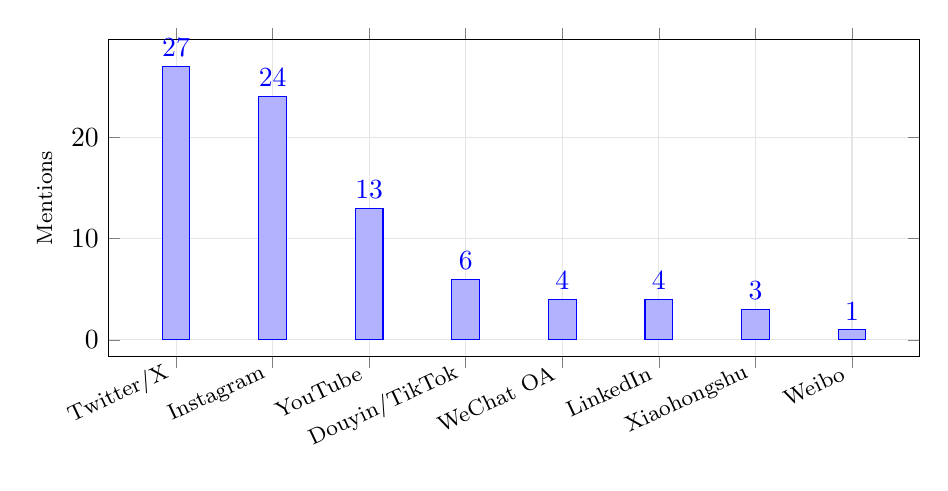
\begin{tikzpicture}
\begin{axis}[
width=0.98\linewidth,
height=5.6cm,
ybar,
ylabel={Mentions},
symbolic x coords={Twitter/X,Instagram,YouTube,Douyin/TikTok,WeChat OA,LinkedIn,Xiaohongshu,Weibo},
xtick=data,
x tick label style={rotate=25, anchor=east, font=\footnotesize},
nodes near coords,
nodes near coords align={vertical},
label style={font=\footnotesize},
grid=major, grid style={draw=gray!20},
every axis plot/.append style={fill=orange!70, draw=orange!80!black},
]
\addplot coordinates {
(Twitter/X,27)
(Instagram,24)
(YouTube,13)
(Douyin/TikTok,6)
(WeChat OA,4)
(LinkedIn,4)
(Xiaohongshu,3)
(Weibo,1)
};
\end{axis}
\end{tikzpicture}
\caption{Platform-related mentions in skill metadata.}
\label{fig:autoskill-platform-bars}
\end{figure}
